\section{Results}
As described earlier the PAN 2013 results are ranked using the F1 measure. The
measure is defined using \textit{precision} and \textit{recall} which in this
case is defined as,

\begin{align}
    precision &=  correct\_answers / answers \\
    recall &= correct\_answers / problems.
\end{align}

Since we answer all problems $problems$ and $answers$ are the same in our case
and we therefore get that the F1 measure is the same as an accuracy,

\begin{equation}
    F1 = 2 \frac{precision \cdot recall}{precision + recall}
        = 2 \frac{accuracy^2}{2accuracy}
        = \frac{2accuracy^2}{2accuracy}
        = \frac{accuracy^2}{accuracy}
        = accuracy.
\end{equation}

Similarly as described earlier the PAN2015 results are ranked using the product
of \gls{AUROC} and c@1. Like F1 in PAN 2015 the c@1 also corresponds to an
accuracy in our case since we answer all questions. The definition of c@1 were,

\begin{equation}
    c@1 = \frac{1}{n} \left(n_c + \frac{n_u \cdot n_c}{n}\right)
\end{equation}

where $n$ is the number of problems, $n_c$ is the number of correct answers and
$n_u$ is the number of unanswered problems. So when $n_u$ is 0 we have,

\begin{equation}
    c@1 = \frac{1}{n} \left(n_c + \frac{n_u \cdot n_c}{n}\right)
        = \frac{1}{n} \left(n_c + \frac{0 \cdot n_c}{n}\right)
        = \frac{1}{n} n_c
        = accuracy.
\end{equation}

In this section we will describe how we have tested our solutions on the test
datasets and give the results of those tests. When we are testing on the PAN
2013 dataset we will report an accuracy as that is the only performance measure.
When we are testing on the PAN 2015 dataset we will report both the \gls{AUROC}
and the accuracy since both are used to measure performance.

\subsection{Delta Method}
The Delta method was tested by creating the same features for both the training
dataset and the test datasets. We then computed the mean and standard variance
of the training set and used that to normalize both the training and test
dataset. For each text in the test dataset we then drew differing numbers of
opposing texts from the training dataset. Those opposing texts were used as the
opposition in the Delta Method. The results for running the delta method on
the two test sets included in PAN 2013 and one dataset included in PAN 2015 is
shown in Table \ref{tab:delta_method_final_results}. The \gls{AUROC} curve for
the Delta Method is shown in Figure \ref{fig:delta_method_roc}. It is created
by computing the \gls{TPR} and \gls{FPR} for the differing number of opposing authors.  
\begin{table}
    \centering
    \begin{tabular}{l|lll}
        \textbf{Opponents} & \textbf{PAN 2013 Test 1} & \textbf{PAN 2013 Test 2}
        & \textbf{PAN 2015 Test} \\ \hline
        1  & 0.58685 & 0.58283 & 0.55870 \\
        2  & 0.62235 & 0.60125 & \textbf{0.56550} \\
        3  & 0.63348 & 0.60771 & 0.53969 \\
        4  & 0.63741 & 0.62173 & 0.52880 \\
        5  & 0.63483 & 0.61897 & 0.52269 \\
        6  & 0.63876 & 0.62787 & 0.52080 \\
        7  & 0.64337 & 0.63188 & 0.51399 \\
        8  & 0.64123 & 0.63488 & 0.51270 \\
        9  & \textbf{0.64438} & 0.63173 & 0.51320 \\
        10 & 0.64235 & \textbf{0.63291} & 0.50840
    \end{tabular}
    \caption{Result of running the delta method on two test sets included in PAN
    2013 and single test set included in PAN 2015 with different number of
    authors. The best score obtained on each dataset is highlighted.}
    \label{tab:delta_method_final_results}
\end{table}

\begin{figure}
    \centering
    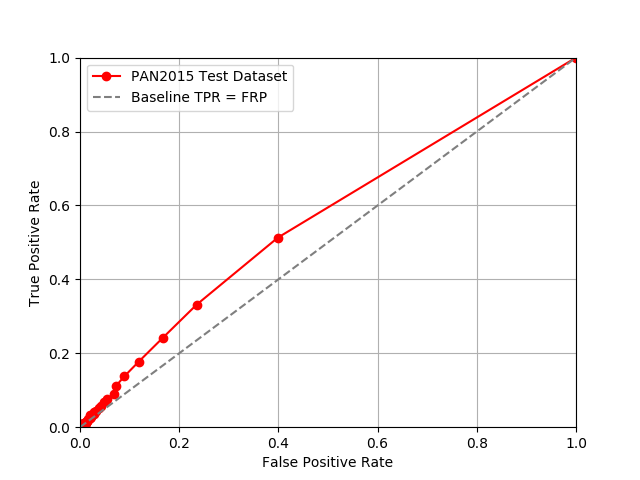
\includegraphics[width=.7\textwidth]{./pictures/delta_method_roc.png}
    \caption{The ROC curve of the delta method with number of opposing authors
    varying from 0 to 10 using the two test datasets for PAN2013 and the test
    dataset for PAN2015.}
    \label{fig:delta_method_roc}
\end{figure}

% TODO: Write how ROC curve were generated.
\subsection{Generalizing Random Forest}
In order to test the universal background approach, proposed by 
\cite{pacheco2015}, a bash script was created which initially

After creating our \gls{UBM} based on the training data and training our random
forest using the two different encodings presented, we got the following
results,

\begin{align}
\text{UBM Enconding Accuracy}:&\qquad 0.604\\
\text{Subtraction Enconding Accuracy}:& \qquad 0.584
\end{align}

\begin{figure}
    \centering
    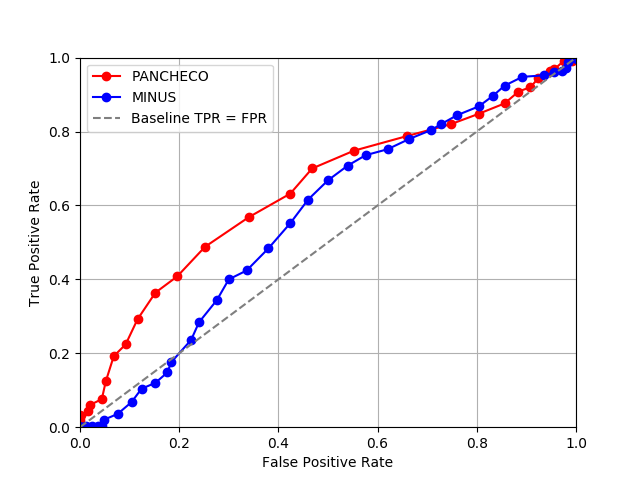
\includegraphics[width=.7\textwidth]{./pictures/forest_roc.png}
    \caption{The ROC curve of the two Generalizing Random Forest approaches.}
    \label{fig:forest_roc}
\end{figure}

\subsection{Extended Delta}
The Extended Delta Method is tested by generating features according to the best
configurations found in the training phase. Then the same procedure used to test
the regular delta method is employed. The best configuration for the PAN 2013
data were the 100 most frequent 2-, 3-, and 4-char-grams and the 300 most
frequent words for 5 opposing authors. The best configuration for the PAN 2015
data were the 20 most frequent 1-, 2-, and 3-special-char-grams for 2 opposing
authors. The accuracy obtained on the PAN 2013 test datasets were 0.73213 and
0.67173. The accuracy obtained on the PAN 2015 dataset were 0.62189. Since the
2015 dataset depends on the \gls{AUROC} it is shown in Figure
\ref{fig:extended_delta_method_roc}.

\begin{figure}
    \centering
    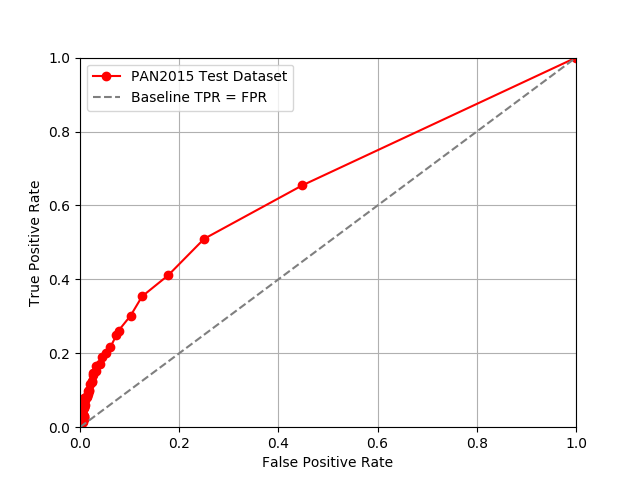
\includegraphics[width=.7\textwidth]{./pictures/extended_delta_method_roc.png}
    \caption{The ROC curve of the Extended Delta Method with number of opposing
    authors varying from 0 to 10 using the test dataset for for PAN2015.}
    \label{fig:extended_delta_method_roc}
\end{figure}

\subsection{Author Specific SVM}
The Author Specific SVM is tested by generating features for the training and
test datasets for the PAN 2013 texts. For each different author in the test
dataset we extract features for all their known texts and their single unknown
text. We then draw random texts from the training dataset which will serve as
opponents to the texts written by the author. Then we train an SVM using the
texts known to be written by the author and the texts from the training dataset
and predict the unknown text using that SVM.

The best configuration on the training set were configuration B using the
frequencies of the 300 most frequent words. On the two test datasets it obtained
accuracies of 0.78650 and 0.78000.

%In the training we tried two different sets of features to train the SVM. They
%both performed about as well as the other and we will therefore
%The accuracy for the two test sets of the PAN 2013 was, 0.85050 and 0.84466.
